
\section[\textlatin{Sets}]{\textgreek{Συνολοθεωρητικές πράξεις}}

\subsection[{\en Union}]{\textgreek{Η σχεσιακή πράξη της ένωσης}}


\begin{frame}[t, fragile, shrink]
\frametitle{Η σχεσιακή πράξη της ένωσης}
\begin{minipage}{\wE}
\large
\begin{block}{Ορισμός της ένωσης:}
  \[
     r \cup s = \{t \,|\, t \in r \; \mathrm{or} \; t \in s \}
  \]
  {\bb Ένωση} δύο σχέσεων $r(R)$ και $s(S)$, που έχουν συμβατότητα τύπου, είναι μια νέα σχέση
  που έχει σχήμα (επικεφαλίδα) ίδιο με αυτό της $r$ και $s$, και κορμό το σύνολο
  των κορμών των $r$ και $s$, δηλαδή όλες τις πλειάδες που ανήκουν στην $r$, ή στην $s$,
  η και στις δύο πλειάδες.
  Η ένωση συμβολίζεται με $r \cup s$  ή $r \quad UNION \quad s$.
\end{block}
\end{minipage}
\end{frame}


\begin{frame}[t, fragile, shrink]
\frametitle{Παράδειγμα ένωσης σχέσεων}
\begin{minipage}{\wE}

\begin{tikzpicture}[thick]
  \filldraw[fill=blue10, fill opacity=0.9]  (-0.7, 0.0) circle (1.2cm);
  \filldraw[fill=blue10, fill opacity=0.9]  ( 0.7, 0.0) circle (1.2cm); 
  \draw[color=black] (-1.0, 0.0) node {1};
  \draw[color=black] (0.0, 0.0) node {2};
  \draw[color=black] (1.0, 0.0) node {3};
  \draw[color=black] (-1.3, 1.3) node {$r$};
  \draw[color=black] (1.3, 1.3) node {$s$};
  \draw (4.15, 1.0)     node {$r = \{1,2\}$};
  \draw (4.15, 0.5)     node {$s = \{2,3\}$};  
  \draw (4.00, 0.0)     node {$r \cup s = \{1,2,3\}$};
\end{tikzpicture}
\pause
\begin{figure}[htp]
\en
\begin{tabular}[t]{ c c c }
  \begin{tabular}{ c c c } \toprule
    {\bf A} & {\bf B} & {\bf C}  \\ \midrule
    1 & b & 10 \\
    5 & a & 30 \\
    3 & c & 20 \\	\bottomrule
      &   &    \\
  \end{tabular} 
&  
  \begin{tabular}{ c c c }  \toprule
    {\bf A} & {\bf B} & {\bf C}  \\ \midrule
    5 & a & 30 \\
    2 & b & 10 \\
    3 & c & 20 \\	\bottomrule
      &   &    \\    
  \end{tabular} 
&  
  \begin{tabular}{ c c c }  \toprule
    {\bf A} & {\bf B} & {\bf C}  \\ \midrule
    1 & b & 10 \\
    5 & a & 30 \\
    3 & c & 20 \\
    2 & b & 10 \\	\bottomrule	
  \end{tabular}
\\  
  $r$ & $s$ & $r \cup s$ \\
\end{tabular}
\el
%\caption{\el Παράδειγμα σχεσιακής ένωσης: $t = r \cup s$}
\label{fig:ra_union_ex1}
\end{figure}
\end{minipage}
\end{frame}


\begin{frame}[t, fragile, shrink]
\frametitle{Ένωση και αντιμεταθετική ιδιότητα}
\begin{minipage}{\wE}
\begin{block}{Ισχύει η αντιμεταθετική ιδιότητα} \Large
    \[ r \cup s = s \cup r \]
\end{block}
\begin{exampleblock}{Παράδειγμα}
\en
\begin{tabular}{ c c c c }
  \begin{tabular}{ c c c } \toprule
    A & B & C \\ \midrule
    1 & b & 10 \\
    5 & a & 30 \\
    3 & c & 20 \\	\bottomrule
  \end{tabular} 
&  
  \begin{tabular}{ c c c }  \toprule
    {\bf A} & {\bf B} & {\bf C}  \\ \midrule
    5 & a & 30 \\
    2 & b & 10 \\
    3 & c & 20 \\	\bottomrule
  \end{tabular} 
&  
  \begin{tabular}{ c c c }  \toprule
    {\bf A} & {\bf B} & {\bf C}  \\ \midrule
    1 & b & 10 \\
    5 & a & 30 \\
    3 & c & 20 \\
    2 & b & 10 \\	\bottomrule	
  \end{tabular}
&  
  \begin{tabular}{ c c c }  \toprule
    {\bf A} & {\bf B} & {\bf C}  \\ \midrule
    5 & a & 30 \\
    2 & b & 10 \\
    3 & c & 20 \\  
    1 & b & 10 \\   \bottomrule	
  \end{tabular}  
\\  
  $r$ & $s$ & $r \cup s$ & $s \cup r$ \\
\end{tabular}
\el
\end{exampleblock}
\end{minipage}
\end{frame}



\begin{frame}[t, fragile, shrink]
\frametitle{Ένωση και προσεταιριστική ιδιότητα}
\begin{minipage}{\wE}
  \begin{block}{Ισχύει η προσεταιριστική ιδιότητα} \Large
    \[ r \cup (s \cup t) = (r \cup s) \cup t \]
  \end{block}
   Λόγω αυτής της της ιδιότητας, είναι δυνατό να γραφεί \\ η παρακάτω παράσταση χωρίς παρενθέσεις:
   \[
     r \cup s \cup t
   \]
   για να δηλώσει την ένωση τριών ή περισσότερων σχέσεων.
\end{minipage}
\end{frame}


\subsection[\textlatin{Difference}]{\textgreek{Η σχεσιακή πράξη της διαφοράς}}

\begin{frame}[t, fragile, shrink]
\frametitle{Η σχεσιακή πράξη της διαφοράς}
\begin{minipage}{\wE}
\large
\begin{block}{Ορισμός της διαφοράς:}
  \[
     r - s = \{t \,|\, t \in r \; \mathrm{and} \; t \notin s \}
  \]
  {\bb Διαφορά} δύο σχέσεων $r(R)$ και $s(S)$, που έχουν συμβατότητα τύπου, είναι μια νέα σχέση
  που έχει σχήμα (επικεφαλίδα) ίδιο με αυτό της $r$ και $s$, και κορμό 
  τις πλειάδες που ανήκουν στην $r$ αλλά όχι στην $s$.
  Η διαφορά συμβολίζεται με $r - s$  ή {\en $r \text{ MINUS }  s$}.
\end{block}
\end{minipage}
\end{frame}


\begin{frame}[t, fragile, shrink]
\frametitle{Παράδειγμα διαφοράς δύο σχέσεων}
\begin{minipage}{\wE}

\begin{tikzpicture}[thick]
  \filldraw[fill=blue90, fill opacity=0.5]  (-0.7, 0.0) circle (1.2cm);
  \filldraw[fill=blue10, fill opacity=0.5]  ( 0.7, 0.0) circle (1.2cm); 
  \draw[color=black] (-1.0, 0.0) node {1};
  \draw[color=black] (0.0, 0.0) node {2};
  \draw[color=black] (1.0, 0.0) node {3};
  \draw[color=black] (-1.3, 1.3) node {$r$};
  \draw[color=black] (1.3, 1.3) node {$s$}; 
  \draw (4.55, 1.0)     node {$r = \{1,2\}$};
  \draw (4.55, 0.5)     node {$s = \{2,3\}$};  
  \draw (4.00, 0.0)     node {$r - s = \{1\}$};
  \draw (4.00,-0.5)     node {$s - r = \{3\}$};  
\end{tikzpicture}
\\
\pause
\par
\large
\en
\begin{tabular}{ c c c c }
  \begin{tabular}{ c c c } \toprule
    {\bf A} & {\bf B} & {\bf C}  \\ \midrule
    1 & b & 10 \\
    5 & a & 30 \\
    3 & c & 20 \\	\bottomrule
  \end{tabular} 
&  
  \begin{tabular}{ c c c }  \toprule
    {\bf A} & {\bf B} & {\bf C}  \\ \midrule
    5 & a & 30 \\
    2 & b & 10 \\
    3 & c & 20 \\	\bottomrule
  \end{tabular} 
&  
  \begin{tabular}{ c c c }  \toprule
    {\bf A} & {\bf B} & {\bf C}  \\ \midrule
    1 & b & 10 \\	\bottomrule
      &   &    \\
      &   &    \\
  \end{tabular}
&  
  \begin{tabular}{ c c c }  \toprule
    {\bf A} & {\bf B} & {\bf C}  \\ \midrule
    2 & b & 10 \\   \bottomrule
      &   &    \\
      &   &    \\    
  \end{tabular}  
\\  
  $r$ & $s$ & $r - s$ & $s - r$ \\
\end{tabular}
\el
\end{minipage}
\end{frame}


\begin{frame}[t, fragile, shrink]
\frametitle{Αντιμεταθετική και προσεταιριστική ιδιότητα}
\begin{minipage}{\wE}
  {\large Στη σχεσιακή πράξη της διαφοράς:}
  \begin{alertblock}{Δεν ισχύει η αντιμεταθετική ιδιότητα}
    \[ r - s \neq s - r \]
  \end{alertblock}
  \begin{alertblock}{Δεν ισχύει η προσεταιριστική ιδιότητα}
    \[ r - (s - t) \neq (r - s) - t \]
  \end{alertblock} 
  \begin{exampleblock}{Υπενθύμιση}
    \[ 5 - 3 \neq 3 - 5 \]
    \[ 8 - (3 - 2) \neq (8 - 3) - 2 \]
  \end{exampleblock}  
\end{minipage}
\end{frame}



\subsection[{\en Intersect}]{\textgreek{Η σχεσιακή πράξη της τομής}}


\begin{frame}[t, fragile, shrink]
\frametitle{Η σχεσιακή πράξη της τομής}
\begin{minipage}{\wE}
\large
\begin{block}{Ορισμός της τομής:}
  \[
     r \cap s = \{t \,|\, t \in r \; \mathrm{and} \; t \in s \}
  \]
  {\bb Τομή} δύο σχέσεων $r(R)$ και $s(S)$, που έχουν συμβατότητα τύπου,
  είναι μια νέα σχέση που έχει σχήμα (επικεφαλίδα) ίδιο με αυτό της $r$ και $s$,
  και κορμό τις πλειάδες που ανήκουν στην $r$ και στην $s$, δηλαδή τις κοινές πλειάδες.
  Η τομή συμβολίζεται με $r \cap s$  ή {\en $r  \text{ INTERSECT } s$}.
\end{block}
\end{minipage}
\end{frame}



\begin{frame}[t, fragile, shrink]
\frametitle{Παράδειγμα τομής δύο σχέσεων}
\begin{minipage}{\wE}

\begin{tikzpicture}[thick]
  \filldraw[fill=blue90, fill opacity=0.5]  (-0.7, 0.0) circle (1.2cm);
  \filldraw[fill=blue10, fill opacity=0.5]  ( 0.7, 0.0) circle (1.2cm); 
  \draw[color=black] (-1.0, 0.0) node {1};
  \draw[color=black] (0.0, 0.0) node {2};
  \draw[color=black] (1.0, 0.0) node {3};
  \draw[color=black] (-1.3, 1.3) node {$r$};
  \draw[color=black] (1.3, 1.3) node {$s$};
  \draw (4.55, 1.0)     node {$r = \{1,2\}$};
  \draw (4.55, 0.5)     node {$s = \{2,3\}$};  
  \draw (4.00, 0.0)     node {$r \cap s = \{2\}$};
\end{tikzpicture}
\\
\pause
\par
\large
\en
\begin{tabular}{ c c c }
  \begin{tabular}{ c c c } \toprule
    {\bf A} & {\bf B} & {\bf C} \\ \midrule
    1 & b & 10 \\
    5 & a & 30 \\
    3 & c & 20 \\   \bottomrule
  \end{tabular}
&
  \begin{tabular}{ c c c }  \toprule
    {\bf A} & {\bf B} & {\bf C} \\ \midrule
    5 & a & 30 \\
    2 & b & 10 \\
    3 & c & 20 \\   \bottomrule
  \end{tabular}
&
  \begin{tabular}{ c c c }  \toprule
    {\bf A} & {\bf B} & {\bf C}  \\ \midrule
    5 & a & 30 \\
    3 & c & 20 \\           \bottomrule
      &   &    \\
  \end{tabular}
\\
  $r$ & $s$ & $r \cap s$ \\
\end{tabular}
\el
\end{minipage}
\end{frame}


\begin{frame}[t, fragile, shrink]
\frametitle{Τομή και αντιμεταθετική ιδιότητα}
\begin{minipage}{\wE}
\begin{block}{Ισχύει η αντιμεταθετική ιδιότητα} \Large
    \[ r \cap s = s \cap r \]
\end{block}
\begin{exampleblock}{Παράδειγμα}
\en
\en
\begin{tabular}{ c c c c }
  \begin{tabular}{ c c c } \toprule
    {\bf A} & {\bf B} & {\bf C} \\ \midrule
    1 & b & 10 \\
    5 & a & 30 \\
    3 & c & 20 \\   \bottomrule
  \end{tabular}
&
  \begin{tabular}{ c c c }  \toprule
    {\bf A} & {\bf B} & {\bf C} \\ \midrule
    5 & a & 30 \\
    2 & b & 10 \\
    3 & c & 20 \\   \bottomrule
  \end{tabular}
&
  \begin{tabular}{ c c c }  \toprule
    {\bf A} & {\bf B} & {\bf C}  \\ \midrule
    5 & a & 30 \\
    3 & c & 20 \\           \bottomrule
      &   &    \\
  \end{tabular}
&
  \begin{tabular}{ c c c }  \toprule
    {\bf A} & {\bf B} & {\bf C}  \\ \midrule
    5 & a & 30 \\
    3 & c & 20 \\           \bottomrule
      &   &    \\    
  \end{tabular}
\\
  $r$ & $s$ & $r \cap s$ & $s \cap r$ \\
\end{tabular}
\el
\el
\end{exampleblock}
\end{minipage}
\end{frame}


\begin{frame}[t, fragile, shrink]
\frametitle{Τομή και προσεταιριστική ιδιότητα}
\begin{minipage}{\wE}
  \begin{block}{Ισχύει η προσεταιριστική ιδιότητα} \Large
    \[ r \cap (s \cap t) = (r \cap s) \cap t \]
  \end{block}
   Λόγω αυτής της της ιδιότητας, είναι δυνατό να γραφεί \\ η παρακάτω παράσταση χωρίς παρενθέσεις:
   \[
     r \cap s \cap t
   \]
   για να δηλώσει την τομή τριών ή περισσότερων σχέσεων.
\end{minipage}
\end{frame}


\begin{frame}[t, fragile, shrink]
\frametitle{Η τομή είναι παράγωγη πράξη}
\begin{minipage}{\wE}
  \begin{block}{Εναλλακτικός ορισμός της τομής} \Large
    \[
       r \cap s = r - (r-s)
    \]
  \end{block}
   Δηλαδή το αποτέλεσμα της τομής $r \cap s$ ισούται με το αποτέλεσμα της διαφοράς
   της $r$ από τη διαφορά $r-s$.
   \begin{exampleblock}{Παράδειγμα}
     Δώστε εσείς ένα παράδειγμα που να επιβεβαιώνει (ή να αναιρεί)
     τον παραπάνω ορισμό.
   \end{exampleblock}
\end{minipage}
\end{frame}


\subsection[{\en Examples}]{\textgreek{Επιπλέον παραδείγματα συνολοθεωρητικών πράξεων}}

\begin{frame}[t, fragile, shrink]
\frametitle{\en Pane Amore}
\begin{minipage}{\wE}
  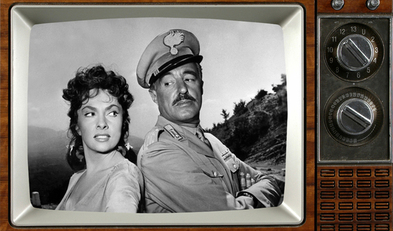
\includegraphics[scale=0.65]{pane-amore.jpg} \\
  \en
  \begin{enumerate}
    \item Pane, amore e fantasia, (1953)
    \item Pane, amore e gelosia, (1954)
    \item Pane, amore e ..., (1955)
  \end{enumerate}
\end{minipage}
\end{frame}

\begin{frame}[t, fragile, shrink]
\frametitle{\en Pane amore}
\begin{minipage}{\wE}
\en
\begin{tabular}{ c c }
  $f$ & $g$ \\
  \begin{tabular}{ c l }              \toprule
    {\bf actorID}  &  {\bf name} \\   \midrule
    0001120  &   Vittorio De Sica \\
    0518178  &   Gina Lollobrigida \\
    0581028  &   Marisa Merlini \\
    0139214  &   Memmo Carotenuto \\
    0728376  &   Roberto Risso \\
    0681365  &   Tina Pica \\
    0188022  &   Vittoria Crispo \\   \bottomrule
  \end{tabular}
  &
  \begin{tabular}{ c l }              \toprule
    {\bf actorID}  &  {\bf name} \\   \midrule
    0001120  &   Vittorio De Sica \\
    0518178  &   Gina Lollobrigida \\
    0581028  &   Marisa Merlini \\
    0139214  &   Memmo Carotenuto \\
    0681365  &   Tina Pica \\
    0882237  &   Saro Urzì \\
    0188022  &   Vittoria Crispo \\     \bottomrule
  \end{tabular}
  \\
\end{tabular}
\el
\end{minipage}
\end{frame}


\begin{frame}[t, fragile, shrink]
\frametitle{{\en Pane amore} (Ερωτήματα συμμετοχής) }
\begin{minipage}{\wE}
  \begin{block}{Έπαιξαν σε τουλάχιστον μία ταινία}
    \[ f \cup g \]
  \end{block}
  \begin{block}{Έπαιξαν και στις δύο πρώτες ταινίες}
    \[ f \cap g \]
  \end{block}
  \begin{block}{Έπαιξαν μόνο στην πρώτη ταινία}
    \[ f - g \]
  \end{block}
  \begin{block}{Έπαιξαν μόνο στη δεύτερη ταινία}
    \[ g - f  \]
  \end{block}
\end{minipage}
\end{frame}



\begin{frame}[t, fragile, shrink]
\frametitle{Τομή {\en fantasia $\cap$ gelosia}}
\begin{minipage}{\wE}
\en
\scriptsize
\begin{tabular}{ c c }
  $f$ & $g$ \\
  \begin{tabular}{ c l }              \toprule
    {\bf actorID}  &  {\bf name} \\   \midrule
    0001120  &   Vittorio De Sica \\
    0518178  &   Gina Lollobrigida \\
    0581028  &   Marisa Merlini \\
    0139214  &   Memmo Carotenuto \\
    0728376  &   Roberto Risso \\
    0681365  &   Tina Pica \\
    0188022  &   Vittoria Crispo \\   \bottomrule
  \end{tabular}
  &
  \begin{tabular}{ c l }              \toprule
    {\bf actorID}  &  {\bf name} \\   \midrule
    0001120  &   Vittorio De Sica \\
    0518178  &   Gina Lollobrigida \\
    0581028  &   Marisa Merlini \\
    0139214  &   Memmo Carotenuto \\
    0681365  &   Tina Pica \\
    0882237  &   Saro Urzì \\
    0188022  &   Vittoria Crispo \\     \bottomrule
  \end{tabular}
  \\
\end{tabular}
\normalsize  \color{blue}
  \begin{tabular}{ c l }              \toprule
    {\bf actorID}  &  {\bf name} \\              \midrule
    0001120  &   Vittorio De Sica \\
    0518178  &   Gina Lollobrigida \\
    0581028  &   Marisa Merlini \\
    0139214  &   Memmo Carotenuto \\ 
    0681365  &   Tina Pica \\     
    0188022  &   Vittoria Crispo \\  \bottomrule
  \end{tabular}
\el
\end{minipage}
\end{frame}


\begin{frame}[t, fragile, shrink]
\frametitle{Διαφορά {\en fantasia $-$ gelosia}}
\begin{minipage}{\wE}
\en
\scriptsize
\begin{tabular}{ c c }
  $f$ & $g$ \\
  \begin{tabular}{ c l }              \toprule
    {\bf actorID}  &  {\bf name} \\   \midrule
    0001120  &   Vittorio De Sica \\
    0518178  &   Gina Lollobrigida \\
    0581028  &   Marisa Merlini \\
    0139214  &   Memmo Carotenuto \\
    0728376  &   Roberto Risso \\
    0681365  &   Tina Pica \\
    0188022  &   Vittoria Crispo \\   \bottomrule
  \end{tabular}
  &
  \begin{tabular}{ c l }              \toprule
    {\bf actorID}  &  {\bf name} \\   \midrule
    0001120  &   Vittorio De Sica \\
    0518178  &   Gina Lollobrigida \\
    0581028  &   Marisa Merlini \\
    0139214  &   Memmo Carotenuto \\
    0681365  &   Tina Pica \\
    0882237  &   Saro Urzì \\
    0188022  &   Vittoria Crispo \\     \bottomrule
  \end{tabular}
  \\
\end{tabular}
\bigskip
\normalsize      \color{blue}
  \begin{tabular}{ c l }              \toprule
    {\bf actorID}  &  {\bf name} \\              \midrule
    0728376  &   Roberto Risso \\  \bottomrule
  \end{tabular}
\el
\end{minipage}
\end{frame}


